\chapter{The crossing tree} % (fold)
\label{cha:the_crossing_tree}

The crossing tree as a tool for analysing self-similarity goes back to the study
of diffusion on fractal sets (see ~\cite{BarlowPerkins88}). It was later reintroduced
by Jones and Shen in \cite{jones2004} in the context of studying self-similarity
and regularity patterns in network traffic data, where it was successfully used in
detecting structural changes, manifested in changes in local regularity of the time
series. In this section I describe theoretical construction of the crossing tree
and how it is recovered from the discrete time series data.

\section{Crossing Times} % (fold)
\label{sec:crossing_times}

Consider a path of real-valued continuous process $\{X(t)\}$ with time running through
$[0,+\infty)$. Continuity is understood in the sense of the path of the process
being almost surely continuous, i.e. the set of discontinuous paths of $\{X(t)\}$
is a subset of a set of probability zero. At the heart of the crossing tree lie
crossing times of a uniformly spaced grid on $\Real$ given by $X(0) + \delta 2^n \mathbb{Z}$
for some $n\geq 0$ and base grid spacing $\delta > 0$.\footnotemark Each $n\geq 0$
represents the ``resolution'' through which sample paths of $\{X(t)\}$ are studied.
\footnotetext{The addition $x_0+A$, for $A$ in an affine space such as $\Real$
represents shifting of every element of the set $A$ by a common value $x_0$.}

In particular, the crossing times $T_k^n$ of process $\{X(t)\}$ at resolution $n\geq 0$
are defined as follows: let $T_0^n = 0$ and for any $k\geq 0$ put
\[
T_{k+1}^n
= \inf \Bigl\{ t \geq T^n_k : \bigr | X(t) - X(T^n_k) \bigr | \geq \delta 2^n \Bigr\}
\]
In other words $T_{k+1}^n$, if it is finite, is the first passage time of a path of
$X(t)$ across a level of $\delta 2^n \mathbb{Z}$ that is different from the line of
the same grid crossed previously. Fixing the zero-th crossing at $0$ automatically
aligns the grid with the process, so in effect, without loss of generality one may
consider processes $X_t$, which start at the origin $X(0)=0$.

By definition, the crossing times of some fixed level $n\geq 0$ are non-decreasing:
$T_k^n \leq T_{k+1}^n$ for all $k\geq 0$. However, since the paths of the process are
almost surely continuous, we show that $T_k^n < T_{k+1}^n$. We proceed by contradiction.
Indeed, by right-continuity of $X(t)$ (a fixed path of $\{X(t)\}$) for $\delta 2^{n-1}$
there is $\eta>0$ with $|X(s)-X(T_k^n)| < \delta 2^{n-1}$ for all $s\in [T_k^n, T_k^n + \eta)$.
However, by definition of $T_{k+1}^n$, in the $\eta$ vicinity of $T_{k+1}^n$,
there exists $\hat{s}$ such that $|X(\hat{s})-X(T_k^n)|\geq \delta 2^n$. Thus, if
$T_k^n = T_{k+1}^n$ then one has $\delta 2^n \leq \delta 2^{n-1}$ -- a contradiction.

Another important property of crossing times is that if $T_{k+1}^n < +\infty$, then
$|X(T_{k+1}^n)-X(T_k^n)| = \delta 2^n$. Indeed, the definition of $T_{k+1}^n$ implies
that there exits a sequence $s_j\downarrow T_{k+1}^n$ with $|X(T_{k+1}^n)-X(T_k^n)|\geq \delta 2^n$
. Since the path $X(t)$ is continuous at $T_{k+1}^n$ it must be true that
\[
|X(T_{k+1}^n)-X(T_k^n)| = \lim_{j\to \infty} |X(s_j)-X(T_k^n)| \geq \delta 2^n\,.
\]
Now, since the function $t\mapsto |X(t)-X(T_k^n)| - \delta 2^n$ is continuous at
$T_{k+1}^n$, $|X(T_{k+1}^n)-X(T_k^n)| > \delta 2^n$ would entail the existence of
$s\in [T_k^n, T_{k+1}^n)$ such that $|X(s)-X(T_k^n)| - \delta 2^n > 0$. This would
contradict the fact that $T_{k+1}^n$ is a lower bound of the set of all $s\geq T_k^n$
with $|X(s)-X(T_k^n)| \geq \delta 2^n$.

So far the crossing times of an almost surely continuous process $\{X(t)\}$, have
the following properties (almost surely): \begin{enumerate}
	\item $T_k^n < T_{k+1}^n$ for all $k\geq 0$;
	\item $|X(T_{k+1}^n)-X(T_k^n)| = \delta 2^n$ for all $k\geq0$ with $T_{k+1}^n<+\infty$.
\end{enumerate}

In order to see the natural tree structure of the crossings, one has to investigate
the properties of the crossing times at different resolutions. We suppose, that for
some integers $k,m\geq 0$, $T_k^n\in [T_m^{n+1}, T_{m+1}^{n+1})$ and $X(T_m^{n+1}) = X(T_k^n)$.

By definition of $T_{k+1}^n$ for all $s\in[T_k^n, T_{k+1}^n)$ it must be true that
\[ |X(s) - X(T_k^n)| < \delta 2^n \,,\]
otherwise $T_{k+1}^n$ would not have been the least lower bound. Since the process
takes the same value at both times $T_m^{n+1}$ and $T_k^n$, it must be true that
$|X(s) - X(T_m^{n+1})| < \delta 2^{n+1}$ for such $s$, whence $s\leq T_{m+1}^{n+1}$.
Therefore $T_{k+1}^n\leq T_{m+1}^{n+1}$.

However, if one further assumes that $T_{m+1}^{n+1} < +\infty$, i.e. that the $(n+1)$-st
crossing takes place, then $T_{k+1}^n \neq T_{m+1}^{n+1}$. Indeed, \begin{itemize}
	\item $|X(T_{k+1}^n)-X(T_k^n)| = \delta 2^n$;
	\item $|X(T_{m+1}^{n+1})-X(T_m^{n+1})| = \delta 2^{n+1}$.
\end{itemize}
together with $X(T_m^{n+1}) = X(T_k^n)$ entail the contradiction $\delta 2^n = \delta 2^{n+1}$.

The assumption that $(n+1)$-level crossing took place (grid $\delta 2^{n+1} \mathbb{Z}$)
allows further refinement of crossing times' behaviour: under the assumptions above,
$T_{k+2}^n\leq T_{m+1}^{n+1}$ holds.

We proceed by contradiction, and suppose otherwise: $T_{m+1}^{n+1} < T_{k+2}^n$.
Then by definition of $T_{k+2}^n$ and because $T_{k+1}^n \leq T_{m+1}^{n+1}$, it
must be true that
\[ |X(T_{m+1}^{n+1}) - X(T_{k+1}^n)| < \delta 2^n \,.\]
However $|X(T_{m+1}^{n+1}) - X(T_m^{n+1})| = \delta 2^{n+1}$ by the established
properties of crossing times on the grid of $n+1$ resolution. Then by the triangle
inequality and the assumption that $X(T_m^{n+1}) = X(T_k^n)$ one gets
\begin{align*}
    |X(T_{m+1}^{n+1}) - X(T_m^{n+1})| 
    & \leq |X(T_{m+1}^{n+1}) - X(T_{k+1}^n)| + |X(T_{k+1}^n) - X(T_m^{n+1})| \\
    & = |X(T_{m+1}^{n+1}) - X(T_{k+1}^n)| + |X(T_{k+1}^n) - X(T_k^n)|\,,
\end{align*}
whence the following contradiction emerges
\[
\delta 2^{n+1}
\leq |X(T_{m+1}^{n+1}) - X(T_{k+1}^n)| + \delta 2^n
< \delta 2^{n+1}\,.
\]
Therefore, under the stated conditions $T_{k+2}^n\leq T_{m+1}^{n+1}$.

%% A nice picture is due here!!!!

% section crossing_times (end)

\section{Tree Structure} % (fold)
\label{sec:tree_structure}

Let's define the \emph{$n$-th level crossing} as the slice of the path of the process
$\{X(t)\}$ over the time half-interval $[T_k^n,T_{k+1}^n)$ for some integer $k\geq 0$,
during which it makes a move of $\pm \delta 2^n$. The uncovered relationship between
crossing times of consecutive levels imply that if $T_k^n \in [T_m^{n+1}, T_{m+1}^{n+1})$
with $X(T_m^{n+1}) = X(T_k^n)$ and $T_{m+1}^{n+1} < +\infty$ then
\[
\bigl[T_k^n,T_{k+1}^n\bigr) \cup \bigl[T_{k+1}^n,T_{k+2}^n\bigr)
\subseteq \bigl[T_m^{n+1},T_{m+1}^{n+1}\bigr) \,.
\]
The first condition, $X(T_m^{n+1}) = X(T_k^n)$ aligns the different resolution grid
with one another. The last requirement that $[T_m^{n+1}, T_{m+1}^{n+1})$ be a finite
interval is natural, since it actually means that the $(n+1)$-st level crossing actually
occurred.

These observations actually state that within the $(n+1)$-st level crossing there musts
be exactly an even number of crossing of the $n$-th level (subcrossings). Indeed,
if $T_k^n = T_m^{n+1}$ and $T_{m+1}^{n+1}<+\infty$, then there are two possibilities
for the crossing time $T_{k+2}^n$: \begin{enumerate}
	\item the process crossed a new level of $(n+1)$-st grid $\delta 2^{n+1}$ in which
	case $T_{m+1}^{n+1}\leq T_{k+2}^n$. Hence there are exactly \emph{two} subcrossings.
	\item the process moved back to the level $X(T_k^n)$, which did not incur a crossing
	of $(n+1)$-st grid, since $X(T_{k+2}^n)=X(T_m^{n+1})$. Yet this fluctuation was
	registered by the grid of resolution $n$. In this case, the properties of crossing
	times entail \[ T_{k+2}^n < T_{k+3}^n < T_{k+4}^n \leq T_{m+1}^{n+1} \,. \]
	Since $T_{m+1}^{n+1}$ is finite, recurrent application of this argument implies that
	there must be exactly an even number of $n$-th level subcrossings in an $(n+1)$-st
	level crossing.
\end{enumerate}
This described behaviour is depicted in figure~\ref{fig:xing_tree_structure}.

%% Draw a simple illustration of the movements within one crossing
\begin{figure}[htb]\begin{center}
    \tikzset{bullet/.style={circle,draw, fill=black,minimum size=5pt,inner sep=0pt},}
    \begin{tikzpicture}[grow=right, sloped]
%% Crossings
        \node [bullet] (o) {};
        \node [bullet] (u) [above right = 3em and 9em of o.west, anchor = west] {};
        \node [bullet] (d) [below right = 3em and 9em of o.west, anchor = west] {};
        \node [bullet] (uu) [above right = 3em and 9em of u.west, anchor = west] {};
        \node [bullet] (ud) [above right = 3em and 9em of d.west, anchor = west] {};
        \node [bullet] (dd) [below right = 3em and 9em of d.west, anchor = west] {};
%% The anchor and labels
        \node [draw=none] [left = 1em of o.west, anchor = east] {$X(T_k^n)$};
        \node [draw=none] [right = 1em of ud.east, anchor = west] {$X(T_k^n)=X(T_{k+2}^n)$};
        \node [draw=none] [right = 1em of uu.east, anchor = west] {$X(T_k^n)+\delta 2^{n+1}$};
        \node [draw=none] [right = 1em of dd.east, anchor = west] {$X(T_k^n)-\delta 2^{n+1}$};
%% Crossing times nodes at the bottom
        \node [draw=none] (t2) [below =of dd.south, anchor = west] {$T_{k+2}^n$};
        \node [draw=none] (t1) [left = 9em of t2.west, anchor = west] {$T_{k+1}^n$};
        \node [draw=none] (t0) [left = 9em of t1.west, anchor = west] {$T_k^n$};
%% Dumy nodes on the top level
        \node [fill=none,draw=none] (dummy2) [above = 1em of uu.north, anchor = north] {};
        \node [fill=none,draw=none] (dummy1) [left = 9em of dummy2.west, anchor = west] {};
        \node [fill=none,draw=none] (dummy0) [left = 9em of dummy1.west, anchor = west] {};
%% Paths to levels
        \path[thick,draw]
            (o) edge node[above] {$+\delta 2^n$} (u)
            (o) edge node[below] {$-\delta 2^n$} (d)
            (u) edge node[above] {$+\delta 2^n$} (uu)
            (u) edge node[below] {$-\delta 2^n$} (ud)
            (d) edge node[above] {$+\delta 2^n$} (ud)
            (d) edge node[below] {$-\delta 2^n$} (dd);
%% Crossing times
        \draw[black, dashed] (dummy2.west -| t2.west) -- (t2.west -| t2.west) {};
        \draw[black, dashed] (dummy1.west -| t1.west) -- (t1.west -| t1.west) {};
        \draw[black, dashed] (dummy0.west -| t0.west) -- (t0.west -| t0.west) {};
    \end{tikzpicture}
%% A very informative caption
    \caption{The structure of possible movements during the crossing $\bigl[T_k^n,T_{k+2}^n\bigr)$.}
\label{fig:xing_tree_structure}
\end{center}\end{figure}

Thus the properties of crossing times of a continuous process permit a natural tree
structure of crossings. If tree levels are enumerated from bottom up then \begin{itemize}
	\item a node at the $(n+1)$-st tree level represents a crossing of the $\delta 2^{n+1} \mathbb{Z}$;
	\item $n$-th level children (offspring) of an $(n+1)$-st level node represent the
	multiple crossings of a finer gird $\delta 2^n \mathbb{Z}$ that took place during
	the larger crossing. 
\end{itemize}

The crossing tree reveals patterns of subcrossings within a parent crossing, conditional
on the direction of the latter. Denote the crossing orientations by
\[ \alpha_k^n = \text{sign}\bigl( X(T_{k+1}^n) - X(T_k^n)\bigr)\,.\]
Then, by construction of the crossing tree itself, subcrossing orientations of a complete
crossing come in pairs by construction. The pairs of oppositely oriented crossings
are \emph{excursions}. Thus orientations (signs) $-+$ and $+-$ correspond to down-up
and up-down excursions, respectively, whereas excursions $--$ or $++$ -- to direct
upward or downward crossings, respectively. Any complete parent crossing can be broken
down into a series of excursions followed by a direct crossing, which actually concludes
the parent crossing by passing over the next $\pm\delta 2^{n+1}$ grid line. Let $V_k^n$
be $0$ if the $k$-th $n$-level excursion (movements within a finer $(n-1)$-st gird) is
up-down (if $\alpha_{2k}^{n-1}\|\alpha_{2k+1}^{n-1} = +-$) and $1$ if it is down-up ($-+$).

The above exposition considered the crossing tree for successively coarser resolutions
$\delta 2^n \mathbb{Z}$ for $n\geq0$. For example in~\cite{decrouez2013estimation} the
crossing tree is defined for crossing times on this grid for any $n\in\mathbb{Z}$.
The restriction to non-negative levels in this paper was motivated by the fact, that
in practice, on real sample path of some supposedly continuous process it is never
possible no meaningfully go beyond some basic finest resolution given by $\delta>0$.
This has to do with the fact that processes are sampled at finite frequency or over
regularly spaced but finitely many points in time. However, it is important to note
that the crossing tree for resolutions finer than the base scale give a one-to-one
characterisation of the original continuous random process in terms of the base scale,
and crossing times $(T_k^n)_{k\geq 0}$ and crossing orientations $(\alpha_k^n)_{k\geq 0}$,
$n\in \mathbb{Z}$ (see~\cite{decrouez2013estimation} and~\cite{ECP1673}).

% section tree_structure (end)

\section{Crossing tree on time series data} % (fold)
\label{sec:crossing_tree_on_time_series_data}

In this section we briefly describe how the crossing tree is constructed for a sample
path of some continuous process, given by time series data $(t_i, x_i)_{i=0}^N$.

In practice the crossing tree is built iteratively from the finest resolution
specified by the base grid spacing $\delta > 0$. The crossing times of the leaves
of the tree are computed for a fixed and given $\delta>0$ in two passes: the first
pass computes passage times on the passed $x_0+\delta \mathbb{Z}$ grid levels, and
the second pass adjusts the passage times and passed levels to eliminate re-crossings
of the same level (recrossing events). The assumption that the time series data
came from a continuous process is the main reason, that enables a sequential procedure
for estimation of the crossing times of grid $\delta\mathbb{Z}$: recall, that
$X(T_{k+1})^n = X(T_k^n) \pm\delta2^n$ if $T_{k+1}^n<\infty$. We refer to the
appendix for details of the procedure.

The choice of $\delta$ is extremely important as it affects the estimates of the
crossing times and levels in the following way, reminiscent of the bias-variance
trade-off:
\begin{itemize}
    \item the grid with too small value of $\delta$ would make the resolution so
    fine as to regard the studied process as a continuous piecewise linear function.
    Each increment would be very likely to produce long consecutive unidirectional
    streaks of crossed levels, which would overestimate the number of crossings
    with only 2 subcrossings by introducing excess number of artificial crossings
    events.
    \item A too large $\delta$ leads to a tree with fewer crossings and offspring,
    which is insufficient for reliable estimates of tree features.
\end{itemize}
One approach to selection of $\delta$ is to consider the increments of the time
series and measure either their standard deviation, or inter-quartile range, or
compute the median of their absolute values. In fact the effect of the base scale
decreases with the level of the tree, provided the tree is tall enough.

% section crossing_tree_on_time_series_data (end)

\section{Analysis using the crossing tree} % (fold)
\label{sec:analysis_using_the_crossing_tree}

Once a crossing tree has been constructed for a particular sample path of a continuous
process $\{X(t)\}$ for a given base resolution $\delta>0$, it can be used to gauge
scale-invariance of the given realisation. Recall that the nodes of level $n$ of
the tree are crossings on the grid $\delta 2^n$, and the offspring of each level
$n+1$ node correspond to the subcrossings of a finer grid $\delta 2^n$ that constitute
the parent crossings. An example of a sample path of a process with superimposed
crossing times and levels is given on figure~\ref{fig:sample_path}. The corresponding
crossing tree is depicted on fig.~\ref{fig:sample_tree}.

\begin{figure}[htb]\begin{center}
    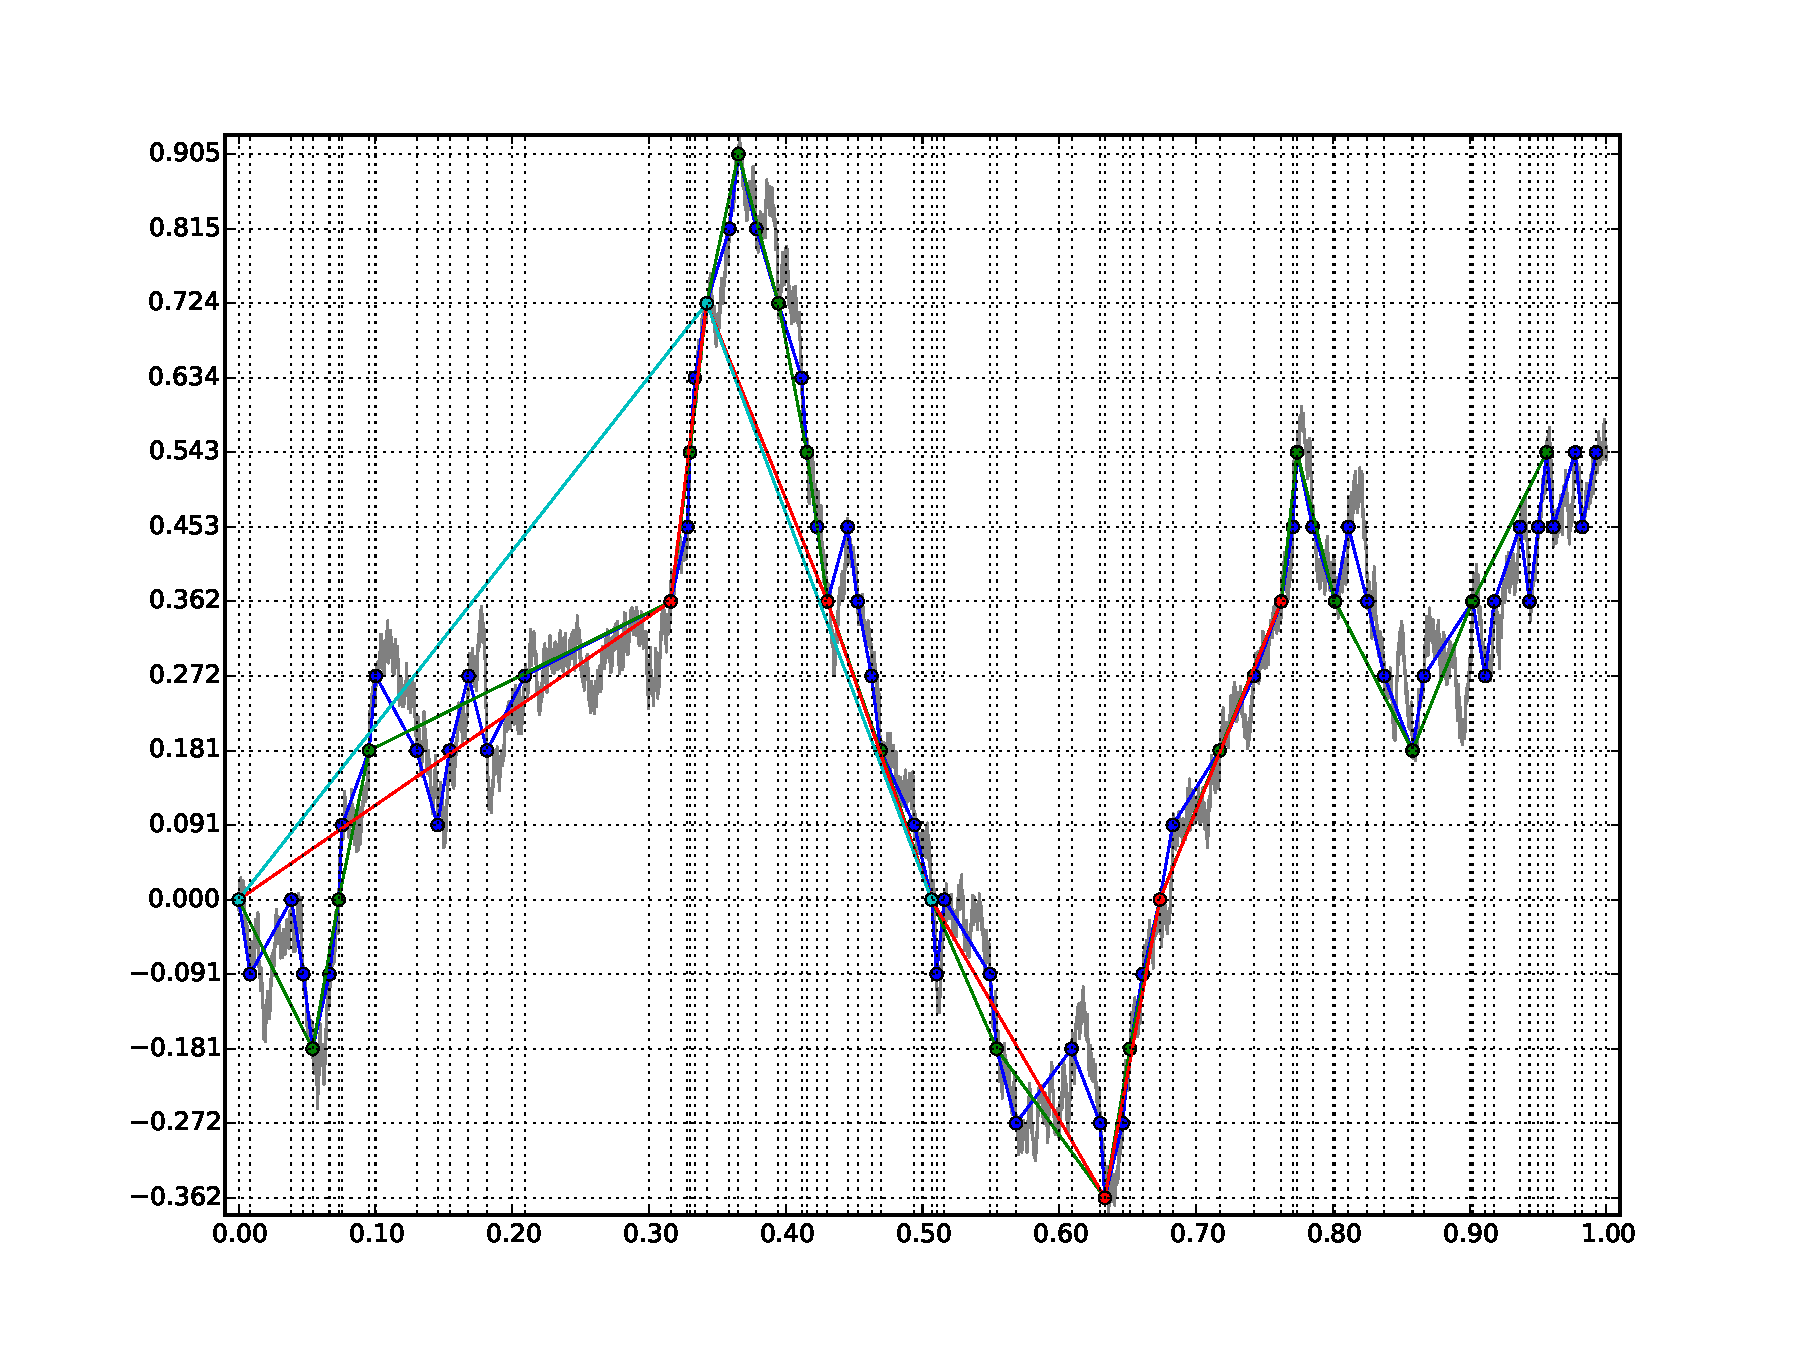
\includegraphics[width=6in]{images/sample_path}
    \caption{The crossing times and levels of a sample trajectory of a continuous process.}
\label{fig:sample_path}
\end{center}\end{figure}
%% Maybe a crossing tree tikz plot should be here...
\begin{figure}[htb]\begin{center}
    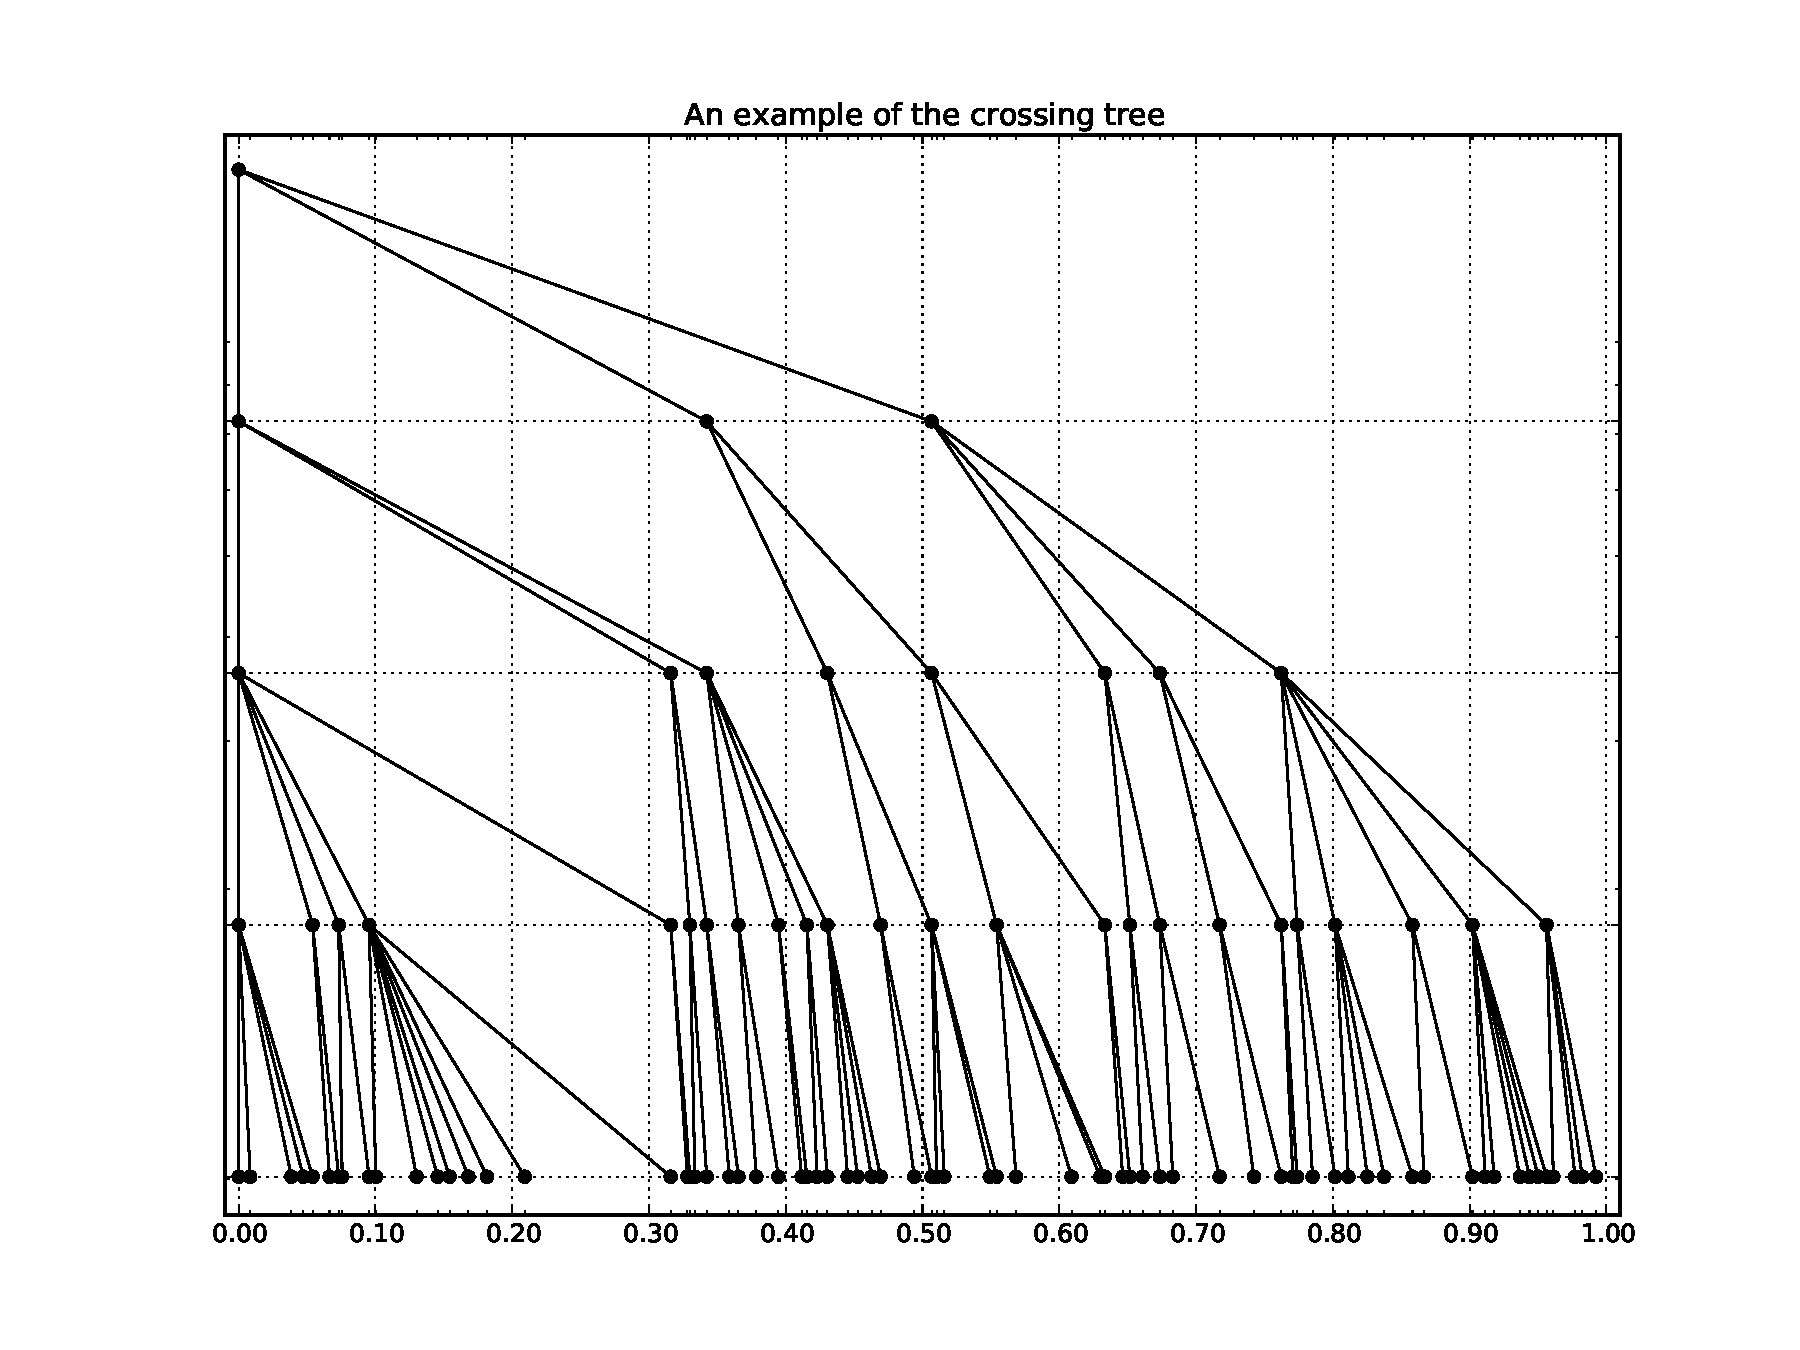
\includegraphics[width=6in]{images/sample_tree}
    \caption{The tree structure of the crossing times for the path depicted in fig.~\ref{fig:sample_path}.}
\label{fig:sample_tree}
\end{center}\end{figure}

Let $Z_k^n$ be the number of subcrossings of a finer grid $\delta 2^{n-1}$ that take
place during the $k$-th crossing of grid $\delta 2^n$, and $N_n$ be the total number
of crossings of level $n$. In general $N_n$ is defined as the last $k\geq0$ such that
$T_k^n < +\infty$. Since it is possible that the very last crossing of the $n$-th
level is incomplete, i.e. the crossing time $T_{N_n}^n = +\infty$, we have the following
inequality:
\[ \sum_{k=1}^{N_{n+1}} Z_k^{n+1} \leq N_n \,.\]
The sequence of numbers of subcrossings, given by $(Z_k)_{k=1}^{N_n}$, can be used to
estimate the offspring distribution. If the process is scale invariant and is ergodic,
it is reasonable to expect that the offspring distributions of crossings of consecutive
levels of the tree are identical, provided the levels are well sampled. To this end one
can use a standard $\chi^2$ squared test: \begin{enumerate}
    \item Take $h$ bins $\{2m\}$ for $m = 1,h-1$ and $\{2h, 2h+2,\ldots\}$ and compute
    the empirical probabilities $\hat{p}_k^n$ of the number of offspring $(Z_k^n)$ on
    each level $n=p, p+1, \ldots, q$ falling into each bin;
    \item Pool all the offspring together into one pool $Z$, and compute the empirical
    probabilities $\bar{p}_i$ of the pooled offspring $Z_k$ being in each of the bins;
    \item Provided each bin has sufficiently many observations, the following statistic
    \[ t^{p,q} = \sum_{j=p}^q \sum_{i=1}^h N_i \frac{(\hat{p}_i^n-\bar{p}_i)^2}{\bar{p}_i} \]
    tests the hypothesis that the offspring distributions on all levels from $p$ to $q$
    have the same distribution. The test statistic has asymptotic $\chi^2$ distribution
    with $(q-p)(h-1)$ degrees of freedom.
\end{enumerate}

Another important characteristic of the process, which is made apparent by the crossing
tree, is the distribution of patterns of subcrossings within a parent crossing, conditional
on its direction. Indeed, subcrossing orientations of a complete crossing come in
pairs by construction of the crossing tree itself: orientations $-+$ and $+-$ correspond
to down-up and up-down excursions respectively, whereas $--$ or $++$ -- to direct
upward or downward crossings. In fact any complete crossing can be broken down
into a series of excursions followed by a direct crossing, which actually end the
current crossing, since they constitute a transitions to a next $\pm\delta 2^{n+1}$
grid line. Let $V_k^n$ be $0$ if the $k$-th $n$-level excursion (movements within a finer
$(n-1)$-st gird) is up-down and $1$ if it is down-up.

If the process is continuous, self-similar and has stationary and ergodic increments
(see~\cite{jonesshen2005}), then the sequences of the number of subcrossings $Z^n = (Z_k^n)_{k\geq 0}$
are identically distributed, stationary and ergodic. The same result holds for
the sequences of properly scaled crossing durations $2^{-n} W^n = (2^{-n} W_k^n)_{k\geq0}$,
where $W_k^n$ is the duration of the $k$-th crossing of level $n$ and is defined
as $W_{k+1}^n = T_{k+1}^n - T_k^n$.

For $H$-sssi processes (see p.\pageref{def:hsssi}) one can use the crossing tree
to estimate the value of the Hurst index $H$ by the following formula:
\[ \hat{H} = \frac{\log 2}{\log \hat{\mu}} \,,\]
where $\hat{\mu} = \ex Z_k^n$. Intuitively, if we one scales the time of an $H$-sssi
process by $\mu$, the expected number of finer subcrossings in a cruder crossing,
then it is necessary to scale down the range of the process by $\tfrac{1}{2}$ --
the multiplier by which the resolution is decreased when ascending the tree from
the finest grid $\delta \mathbb{Z}$. In practice, in order to improve the accuracy of
this estimate one attempts to pool sequences $Z^n$ across several consecutive levels
of the tree, over which the hypothesis of common distribution cannot be rejected.

% section analysis_using_the_crossing_tree (end)

\section{The crossing tree of Brownian motion} % (fold)
\label{sec:the_crossing_tree_of_brownian_motion}

One of most well studied processes is the Brownian motion. Usually it is axiomatically
as a unique stochastic process $\bigl\{W(t)\bigr\}$ with the following four properties:
\begin{itemize}
    \item $W(t)$ is almost surely $0$ at $t=0$;
    \item $\{W(t)\}$ has independent and stationary increments;
    \item for all $t\geq 0$ the random variable $W(t)$ has Gaussian distribution with
    parameters mean $0$ and variance $t$;
    \item the sample paths of $\{W(t)\}$ are almost surely continuous functions.
\end{itemize}
This process exhibits scale-invariance properties, or self-similarity, since for any
$a>0$, the process $\bigl\{a^{-\tfrac{1}{2}} B(at)\bigr\}$ and $\{B(t)\}$ are stochastically
equivalent in the sense of equality of all their finite-dimensional joint distributions.

The paper \cite{ECP1673} gives a rigorous proof of the statistical properties of
the offspring distribution, crossing lengths and the excursions for crossing trees
built over paths of Brownian motion. Theorem 1 of~\cite{ECP1673}, p.~640, states
that the Brownian motion is the unique continuous process $\{B(t)\}$ for which the
crossing tree has infinitely many offspring at each level ($N_n = +\infty$), and:
\begin{description}
    \item[BM0] $B(0) = 0$;
    \item[BM1] the properly scaled crossing durations $\delta^{-2} 4^{-\sfrac{n}{2H}} W_k^n$
    for $H = \tfrac{1}{2}$ are identically distributed with mean 1 and finite variance,
    and are mutually independent within each level $n$;
    \item[BM2] the random variables $Z_k^n$ are iid with probability distribution
    \[ \pr\bigl(Z_k^n=2m\bigr) = 2^{1-H^{-1}}\bigl(1-2^{1-(\sfrac{1}{2})^{-1}}\bigr)^{m-1} \,,\]
    for all $m=1,2,\ldots$;
    \item[BM3] the excursions $V_k^n$ are also iid random variables with 
    $\pr( V_k^n = 1 ) = 2^{-2H^{-1}}$, for $H = \tfrac{1}{2}$.
    $\text{Bern}(\tfrac{1}{2})$.
\end{description}
This theorem crucially depends on the strong Markov property of Bm, which makes $Z_k^n$
independent random variables. The characterisation of Brownian motion in terms of
the properties of its crossing tree is based on ideas used in the construction of
Brownian motion on a nested fractal (see~\cite{BarlowPerkins88}).

% section the_crossing_tree_of_brownian_motion (end)

% chapter the_crossing_tree (end)
